\documentclass[12pt, letterpaper, onecolumn, conference, final]{IEEEtran}

\usepackage[margin = .5in]{geometry}
\usepackage{amsmath}
\usepackage{amsthm}
\usepackage{amssymb}
\usepackage{wasysym}
\usepackage{graphicx}
\usepackage[makeroom]{cancel}
\usepackage{polynom}
\usepackage{booktabs}

\title{Rotations \& Quaternions}
\author{Nathan Marianovsky}

\theoremstyle{definition}
\newtheorem{definition}{Definition}
\newtheorem{proposition}{Proposition}

\theoremstyle{plain}
\newtheorem{theorem}{Theorem}[section]
\newtheorem{example}{Example}
\newtheorem{solution}{Solution}

\renewcommand{\qedsymbol}{$\blacksquare$}

\renewcommand\thesection{\arabic{section}}

\begin{document}

\maketitle

\section*{\underline{\textbf{Crash Course on Groups}}}
\vspace{.3cm}
\begin{center}
\fbox{
\begin{minipage}{7.3 in}
\begin{definition}[Group] 
A \textit{group}, $G$, is a set with a binary operation, $*$, commonly written as $G(S, *)$ where $S$ is the set. All groups adhere to the four axioms:
\begin{itemize}

\item[(1)]
Closure:
\begin{equation*}
\forall x,y \in G: \hspace{.2cm} x*y \in G
\end{equation*}

\item[(2)]
Associativity:
\begin{equation*}
\forall x,y,z \in G: \hspace{.2cm} (a*b)*c = a*(b*c)
\end{equation*}

\item[(3)]
Identity:
\begin{equation*}
\exists! \hspace{.1cm} e \in G \hspace{.2cm} \text{s.t.} \hspace{.2cm} \forall x \in G: \hspace{.2cm} x*e = e*x = x
\end{equation*}

\item[(4)]
Inverse:
\begin{equation*}
\forall x \in G, \hspace{.1cm} \exists y \in G \hspace{.2cm} \text{s.t.} \hspace{.2cm} x*y = y*x = e
\end{equation*}

\end{itemize}
\end{definition}
\end{minipage}}
\end{center}

\noindent
Some common groups where the objects of interest are matrices and the binary operation is matrix multiplication include, but are not limited to:
\begin{center}
\begin{itemize}

\item[(1)]
General Linear:
\begin{equation*}
\textbf{GL}(n,F) = \{ A \in F^{n^2} \hspace{.1cm} | \hspace{.1cm} \det(A) \neq 0 \}
\end{equation*}

\item[(2)]
Special Linear:
\begin{equation*}
\textbf{SL}(n,F) = \{ A \in F^{n^2} \hspace{.1cm} | \hspace{.1cm} \det(A) = 1 \}
\end{equation*}

\item[(3)]
Orthogonal:
\begin{equation*}
\textbf{O}(n,F) = \{ A \in F^{n^2} \hspace{.1cm} | \hspace{.1cm} A^{-1} = A^T \}
\end{equation*}

\item[(4)]
Special Orthogonal:
\begin{equation*}
\textbf{SO}(n,F) = \{ A \in F^{n^2} \hspace{.1cm} | \hspace{.1cm} A^{-1} = A^T \& \det(A) = 1 \}
\end{equation*}

\item[(5)]
Unitary:
\begin{equation*}
\textbf{U}(n,F) = \{ A \in F^{n^2} \hspace{.1cm} | \hspace{.1cm} A^{-1} = A^\dagger \}
\end{equation*}

\item[(6)]
Special Unitary:
\begin{equation*}
\textbf{SU}(n,F) = \{ A \in F^{n^2} \hspace{.1cm} | \hspace{.1cm} A^{-1} = A^\dagger \& \det(A) = 1 \}
\end{equation*}

\item[(7)]
Symplectic:
\begin{equation*}
\textbf{Sp}(2n,F) = \Bigg\{ A \in F^{4n^2} \hspace{.1cm} | \hspace{.1cm} A^T\Omega A = \Omega \hspace{.1cm} \text{where} \hspace{.1cm} \Omega = \begin{pmatrix}
0 & I_n \\
-I_n & 0
\end{pmatrix} \Bigg\}
\end{equation*}

\end{itemize}
\end{center}
where $n$ is the parameter referring to $A$ being a $n \times n$ matrix and $F$ is the field. Typical fields of interest include the integers, real numbers, and complex numbers.

\newpage
\section*{\underline{\textbf{Quaternions}}}
\vspace{.3cm}
\begin{center}
\fbox{
\begin{minipage}{7.3 in}
\begin{definition}[Quaternion] 
A \textit{quaternion} is any number that can be written as:
\begin{equation*}
q = a + bi + cj + dk \hspace{.2cm} \text{where} \hspace{.2cm} a,b,c,d \in \mathbb{R}
\end{equation*}
where $a$ is known as the real part and the rest denotes the imaginary part. Along with this we have:
\begin{equation*}
\begin{split}
i^2 = j^2 &= k^2 = -1 \\
ij = k \hspace{.2cm} &\text{and} \hspace{.2cm} ji = -k \\
jk = i \hspace{.2cm} &\text{and} \hspace{.2cm} kj = -i \\
ki = j \hspace{.2cm} &\text{and} \hspace{.2cm} ik = -j
\end{split}
\end{equation*}
Obviously the above is a pain to remember, so instead you can use the cycle below to remember how the multiplication works where reversing the direction throws in a negative sign:
\begin{center}
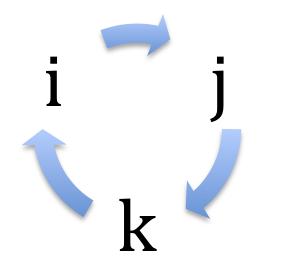
\includegraphics[scale=.3]{Quaternion_Algebra.png}
\end{center}
Note that while real and complex numbers are commutative, quaternions in general are not. In addition any quaternion that has a zero valued real part is known as a \textit{pure imaginary quaternion}.
\end{definition}
\end{minipage}}
\end{center}

\begin{center}
\fbox{
\begin{minipage}{7.3 in}
\begin{proposition}[Relation to $\mathbb{R}^3$ Vector Operations] 
Given any two quaternions that are written down into separate real and imaginary components as:
\begin{equation*}
p = p_0 + \overrightarrow{p} \hspace{.2cm} \text{and} \hspace{.2cm} q = q_0 + \overrightarrow{q}
\end{equation*}
their multiplication is defined as:
\begin{equation*}
pq = (p_0q_0 - \overrightarrow{p} \cdot \overrightarrow{q}) + (p_0\overrightarrow{q} + q_0\overrightarrow{p} + \overrightarrow{p} \times \overrightarrow{q})
\end{equation*}
where $\cdot$ and $\times$ represent the standard dot product and cross product on $\mathbb{R}^3$ respectively.
\end{proposition}
\end{minipage}}
\end{center}

\begin{proof}
We start by defining the quaternions as:
\begin{equation*}
p = p_0 + p_1i + p_2j + p_3k \hspace{.2cm} \text{and} \hspace{.2cm} q = q_0 + q_1i + q_2j + q_3k
\end{equation*}
Now multiplying them gives:
\begin{equation*}
\begin{split}
pq &= (p_0 + p_1i + p_2j + p_3k)(q_0 + q_1i + q_2j + q_3k) \\
&= (p_0q_0 + p_1q_1i^2 + p_2q_2j^2 + p_3q_3k^2) + p_0q_1i + p_0q_2j + p_0q_3k + p_1q_0i \\
& \hspace{.4cm} + p_1q_2ij + p_1q_3ik + p_2q_0j + p_2q_1ji + p_2q_3jk + p_3q_0k + p_3q_1ki + p_3q_2kj \\
&= (p_0q_0 - p_1q_1 - p_2q_2 - p_3q_3) + p_0q_1i + p_0q_2j + p_0q_3k + p_1q_0i \\
& \hspace{.4cm} + p_1q_2k - p_1q_3j + p_2q_0j - p_2q_1k + p_2q_3i + p_3q_0k + p_3q_1j - p_3q_2i \\
&= (p_0q_0 - p_1q_1 - p_2q_2 - p_3q_3) + p_0(q_1i + q_2j + q_3k) + q_0(p_1i + p_2j + p_3k) \\
& \hspace{.4cm} + \Big[ (p_2q_3 - p_3q_2)i + (p_3q_1 - p_1q_3)j + (p_1q_2 - p_2q_1)k \Big]
\end{split}
\end{equation*}
If we vectorize the imaginary component of each quaternion as:
\begin{equation*}
\overrightarrow{p} = p_1i + p_2j + p_3k \hspace{.2cm} \text{and} \hspace{.2cm} \overrightarrow{q} = q_1i + q_2j + q_3k
\end{equation*}
then the multiplication takes on the form:
\begin{equation*}
pq = (p_0q_0 - \overrightarrow{p} \cdot \overrightarrow{q}) + (p_0\overrightarrow{q} + q_0\overrightarrow{p} + \overrightarrow{p} \times \overrightarrow{q})
\end{equation*}
\end{proof}

\newpage
\begin{center}
\fbox{
\begin{minipage}{7.3 in}
\begin{definition}[Conjugation] 
Similar to complex numbers, the conjugate of any given quaternion:
\begin{equation*}
q = q_0 + q_1i + q_2j + q_3k
\end{equation*}
is defined as:
\begin{equation*}
q^* = q_0 - q_1i - q_2j - q_3k
\end{equation*}
Notice that by multiplying the two we arrive at:
\begin{equation*}
\| q \|^2 = qq^* = q^*q = q_0^2 + q_1^2 + q_2^2 + q_3^2
\end{equation*}
which defines the square of the norm for any given quaternion.
\end{definition}
\end{minipage}}
\end{center}

\begin{center}
\fbox{
\begin{minipage}{7.3 in}
\begin{proposition}[Redefining the Dot and Cross Products of $\mathbb{R}^3$] 
Take two pure imaginary quaternions:
\begin{equation*}
p = p_1i + p_2j + p_3k \hspace{.2cm} \text{and} \hspace{.2cm} q = q_1i + q_2j + q_3k
\end{equation*}
We can now define the dot and cross products as:
\begin{equation*}
\begin{split}
p \cdot q &= \frac{1}{2}(p^*q + q^*p) = \frac{1}{2}(pq^* + qp^*) \\
p \times q &= \frac{1}{2}(pq - q^*p^*)
\end{split}
\end{equation*}
\end{proposition}
\end{minipage}}
\end{center}

\begin{proof}
To begin consider the fact that for any two quaternions $p$ and $q$ we have:
\begin{equation*}
pq = (p_0q_0 - \overrightarrow{p} \cdot \overrightarrow{q}) + (p_0\overrightarrow{q} + q_0\overrightarrow{p} + \overrightarrow{p} \times \overrightarrow{q})
\end{equation*}
Now if we want to talk about pure imaginary quaternions we set $p_0 = q_0 = 0$ to get:
\begin{equation*}
pq = \overrightarrow{p} \times \overrightarrow{q} - \overrightarrow{p} \cdot \overrightarrow{q}
\end{equation*}
With this can now define:
\begin{equation*}
\begin{split}
p^*q &= (-\overrightarrow{p}) \times \overrightarrow{q} - (-\overrightarrow{p}) \cdot \overrightarrow{q} \\
&= -\overrightarrow{p} \times \overrightarrow{q} + \overrightarrow{p} \cdot \overrightarrow{q} \\
q^*p &= (-\overrightarrow{q}) \times \overrightarrow{p} - (-\overrightarrow{q}) \cdot \overrightarrow{p} \\
&= \overrightarrow{p} \times \overrightarrow{q} + \overrightarrow{p} \cdot \overrightarrow{q}
\end{split}
\end{equation*}
Adding these two together and isolating the dot product gives:
\begin{equation*}
\begin{split}
2\overrightarrow{p} \cdot \overrightarrow{q} &= p^*q + q^*p \\
\overrightarrow{p} \cdot \overrightarrow{q} &= \frac{1}{2}(p^*q + q^*p)
\end{split}
\end{equation*}
I now remind you that the dot product will always give back a real number, therefore conjugation will not change the result and so:
\begin{equation*}
\begin{split}
(\overrightarrow{p} \cdot \overrightarrow{q})^* &= \Big[ \frac{1}{2}(p^*q + q^*p) \Big]^* \\
\overrightarrow{p} \cdot \overrightarrow{q} &= \frac{1}{2}(pq^* + qp^*)
\end{split}
\end{equation*}
where the conjugation of the product is equivalent to the product of the conjugations in the same order. Lastly we define:
\begin{equation*}
\begin{split}
q^*p^* &= (-\overrightarrow{q}) \times (-\overrightarrow{p}) - (-\overrightarrow{q}) \cdot (-\overrightarrow{p}) \\
&= -\overrightarrow{p} \times \overrightarrow{q} - \overrightarrow{p} \cdot \overrightarrow{q} \\
\end{split}
\end{equation*}
and subtract it from the original multiplication to arrive at the definition of the cross product:
\begin{equation*}
\begin{split}
2\overrightarrow{p} \times \overrightarrow{q} &= pq - q^*p^* \\
\overrightarrow{p} \times \overrightarrow{q} &= \frac{1}{2}(pq - q^*p^*)
\end{split}
\end{equation*}
\end{proof}

\newpage
\begin{center}
\fbox{
\begin{minipage}{7.3 in}
\begin{definition}[Matrix Representations] 
Any given quaternion:
\begin{equation*}
q = q_0 + q_1i + q_2j + q_3k
\end{equation*}
can be written as a $2 \times 2$ matrix with inputs consisting of complex numbers:
\begin{equation*}
q = \begin{pmatrix}
q_0 + q_1i & q_2 + q_3i \\
-q_2 + q_3i & q_0 - q_1i
\end{pmatrix}
\end{equation*}
If you do not happen to like imaginary components, then this definition can be easily rewritten as a $4 \times 4$ matrix consisting of real numbers as:
\begin{equation*}
q = \begin{pmatrix}
q_0 & q_1 & q_2 & q_3 \\
-q_1 & q_0 & -q_3 & q_2 \\
-q_2 & q_3 & q_0 & -q_1 \\
-q_3 & -q_2 & q_1 & q_0
\end{pmatrix}
\end{equation*}
\end{definition}
\end{minipage}}
\end{center}

\begin{center}
\fbox{
\begin{minipage}{7.3 in}
\begin{proposition}[Conjugate in Matrix Representation] 
If we represent a quaternion as a matrix, then the conjugate of the quaternion is equivalent to the conjugate transpose of the matrix.
\end{proposition}
\end{minipage}}
\end{center}

\begin{proof}
Let us define:
\begin{equation*}
\begin{split}
q &= q_0 + q_1i + q_2j + q_3k \\
q^* &= q_0 - q_1i - q_2j - q_3k
\end{split}
\end{equation*}
where we know that:
\begin{equation*}
q = \begin{pmatrix}
q_0 + q_1i & q_2 + q_3i \\
-q_2 + q_3i & q_0 - q_1i
\end{pmatrix}
\end{equation*}
Now to define the conjugate in terms of a matrix, just place a negative sign in front of the imaginary components:
\begin{equation*}
q^* = \begin{pmatrix}
q_0 - q_1i & -q_2 - q_3i \\
q_2 - q_3i & q_0 + q_1i
\end{pmatrix}
\end{equation*}
which is equivalent to:
\begin{equation*}
q^* = \Bigg[ \begin{pmatrix}
q_0 + q_1i & q_2 + q_3i \\
-q_2 + q_3i & q_0 - q_1i
\end{pmatrix} \Bigg]^\dagger = \begin{pmatrix}
q_0 - q_1i & -q_2 - q_3i \\
q_2 - q_3i & q_0 + q_1i
\end{pmatrix}
\end{equation*}
\end{proof}

\begin{center}
\fbox{
\begin{minipage}{7.3 in}
\begin{proposition}[Norm in Matrix Representation] 
If we represent a quaternion as a matrix, then the norm squared of the quaternion is equivalent to the determinant of the matrix.
\end{proposition}
\end{minipage}}
\end{center}

\begin{proof}
We note that the square of the norm is already defined as:
\begin{equation*}
\| q \|^2 = q_0^2 + q_1^2 + q_2^2 + q_3^2
\end{equation*}
Now taking the determinant of the matrix representation gives:
\begin{equation*}
\begin{split}
\| q \|^2 &= \det \begin{pmatrix}
q_0 + q_1i & q_2 + q_3i \\
-q_2 + q_3i & q_0 - q_1i
\end{pmatrix} \\
&= (q_0 + q_1i)(q_0 - q_1i) - (q_2 + q_3i)(-q_2 + q_3i) \\
&= q_0^2 + q_1^2 + q_2^2 + q_3^2
\end{split}
\end{equation*}
\end{proof}

\newpage
\begin{center}
\fbox{
\begin{minipage}{7.3 in}
\begin{definition}[Unit Quaternions] 
Any quaternion $q$ that has a norm equivalent to exactly $1$ is known as a \textit{unit quaternion}.
\end{definition}
\end{minipage}}
\end{center}

\begin{center}
\fbox{
\begin{minipage}{7.3 in}
\begin{proposition}[Generating a Unit Quaternion] 
In general given any arbitrary quaternion, $q$, we can generate a unit quaternion by dividing by the norm:
\begin{equation*}
q_u = \frac{q}{\| q \|}
\end{equation*}
\end{proposition}
\end{minipage}}
\end{center}

\begin{proof}
To check we just have to see that the norm of the new quaternion is actually equivalent to $1$:
\begin{equation*}
\begin{split}
\| q_u \| &= \sqrt{q_uq_u^*} \\
&= \sqrt{\Big( \frac{q}{\| q \|} \Big) \Big( \frac{q^*}{\| q \|} \Big)} \\
&= \sqrt{\frac{qq^*}{\| q \|^2}} \\
&= \sqrt{\frac{qq^*}{qq^*}} \\
&= 1
\end{split}
\end{equation*}
\end{proof}

\begin{center}
\fbox{
\begin{minipage}{7.3 in}
\begin{proposition}[Quaternion Reciprocal] 
A quaternion reciprocal can always be defined as:
\begin{equation*}
q^{-1} = \frac{q^*}{\| q \|^2} \hspace{.2cm} \text{s.t.} \hspace{.2cm} q^{-1}q = qq^{-1} = 1
\end{equation*}
so long as $q \neq 0$.
\end{proposition}
\end{minipage}}
\end{center}

\begin{proof}
In general since quaternions are not commutative, there should exist a distinction between the left and right inverse. Fortunately the definition above abuses the unit quaternions in a way s.t. both inverses are equivalent. To show this just multiply out $q$ with its inverse in both directions to arrive at the same result:
\begin{equation*}
\begin{split}
q^{-1}q &= \Big( \frac{q^*}{\| q \|^2} \Big) q = \frac{q^*q}{\| q \|^2} = 1 \\
qq^{-1} &= q \Big( \frac{q^*}{\| q \|^2} \Big) = \frac{qq^*}{\| q \|^2} = 1
\end{split}
\end{equation*}
\end{proof}

\begin{center}
\fbox{
\begin{minipage}{7.3 in}
\begin{proposition}[Quaternion Representation of $\textbf{S}^3$] 
Pure imaginary quaternions with norm equivalent to $1$ form a group isomorphic to $\textbf{S}^3$ with the binary operation of quaternion multiplication.
\end{proposition}
\end{minipage}}
\end{center}

\begin{proof}
We have to check the four conditions for being a group:
\begin{itemize}

\item[(1)]
We know that multiplying any two quaternions together yields another quaternion. As an add on we also know that if both of the original quaternions have norm equivalent to $1$, then so will the final result:
\begin{equation*}
\| q_3 \| = \| q_1q_2 \| = \| q_1 \| \| q_2 \| = (1)(1) = 1
\end{equation*}
where the modulus is allowed to be split up under multiplication same as the complex case.

\item[(2)]
Even though quaternions are not commutative, it is known that they are associative.

\item[(3)]
As for the identity we can define it to be:
\begin{equation*}
e = 1
\end{equation*}

\item[(4)]
The inverse we define to be the conjugate:
\begin{equation*}
q^{-1} = \frac{q^*}{\| q \|^2} = q^*
\end{equation*}
since the norm is taken to be $1$.

\end{itemize}
\end{proof}

\newpage
\begin{center}
\fbox{
\begin{minipage}{7.3 in}
\begin{proposition}[Useful Identity] 
Given a pure imaginary quaternion, $q$, we have the following identity:
\begin{equation*}
q^{2n} = (-1)^n \| q \|^{2n} \hspace{.2cm} \text{where} \hspace{.2cm} n \in \mathbb{Z}^+
\end{equation*}
\end{proposition}
\end{minipage}}
\end{center}

\begin{proof}
This can easily be proved by induction. For the base case consider $n = 0$ which gives:
\begin{equation*}
\begin{split}
q^{0} &= (-1)^0 \| q \|^{0} \\
1 &= 1
\end{split}
\end{equation*}
Now we assume that the statement holds true for $n$ and try to show that it holds for $n+1$:
\begin{equation*}
\begin{split}
q^{2(n + 1)} &= q^{2n + 2} \\
&= q^{2n}q^2 \\
&= (-1)^n \| q \|^{2n}q^2 \\
&= (-1)^{n+1} \| q \|^{2n} (q)(-q) \\
&= (-1)^{n+1} \| q \|^{2n} (q)(q^*) \\
&= (-1)^{n+1} \| q \|^{2n} \| q \|^2 \\
&= (-1)^{n+1} \| q \|^{2n + 2} \\
&= (-1)^{n+1} \| q \|^{2(n + 1)}
\end{split}
\end{equation*}
\end{proof}

\begin{center}
\fbox{
\begin{minipage}{7.3 in}
\begin{proposition}[Euler's Formula] 
Given a quaternion:
\begin{equation*}
p = e^q
\end{equation*}
where $q$ is pure imaginary, we can rewrite $p$ as:
\begin{equation*}
p = \cos\| q \| + \frac{q}{\| q \|}\sin\| q \|
\end{equation*}
A consequence of this setup forces $p$ to be a unit quaternion.
\end{proposition}
\end{minipage}}
\end{center}

\begin{proof}
To begin we know that we can expand the exponential as a power series and using the above identity we arrive at:
\begin{equation*}
\begin{split}
p &= \sum_{n = 0}^\infty \frac{q^n}{n!} \\
&= \sum_{n = 0}^\infty \frac{q^{2n}}{(2n)!} + \sum_{n = 0}^\infty \frac{q^{2n + 1}}{(2n + 1)!} \\
&= \sum_{n = 0}^\infty \frac{(-1)^n \| q \|^{2n}}{(2n)!} + \sum_{n = 0}^\infty \frac{(-1)^n \| q \|^{2n} q}{(2n + 1)!} \\
&= \sum_{n = 0}^\infty \frac{(-1)^n \| q \|^{2n}}{(2n)!} + \frac{q}{\| q \|} \sum_{n = 0}^\infty \frac{(-1)^n \| q \|^{2n + 1}}{(2n + 1)!} \\
&= \cos\| q \| + \frac{q}{\| q \|}\sin\| q \|
\end{split}
\end{equation*}
Now if we want to check the norm of $p$ we have:
\begin{equation*}
\begin{split}
\| p \| &= \sqrt{pp^*} \\
&= \sqrt{(e^q)(e^q)^*} \\
&= \sqrt{(e^q)(e^{q^*})} \\
&= \sqrt{(e^q)(e^{-q})} \\
&= 1
\end{split}
\end{equation*}
\end{proof}

\newpage
\section*{\underline{\textbf{Rotations}}}
\vspace{.3cm}
\begin{center}
\fbox{
\begin{minipage}{7.3 in}
\begin{proposition}[Rodrigues' Rotation Formula] 
Given a vector $v \in \mathbb{R}^3$ and a unit vector $\hat{k} \in \mathbb{R}^3$ describing an axis of rotation about which $v$ rotates by an angle $\theta$, according to the right hand rule the resulting vector after rotation is defined as:
\begin{equation*}
v' = \cos(\theta)v + \sin(\theta)(\hat{k} \times v) + (1 - \cos(\theta))(\hat{k} \cdot v)\hat{k}
\end{equation*}
This result is known as Rodrigues' Rotation Formula.
\end{proposition}
\end{minipage}}
\end{center}

\begin{proof}
To begin take the vector we want to rotate and split it into components relative to the axis $\hat{k}$:
\begin{equation*}
v = v_\perp + v_\parallel
\end{equation*}
where the parallel component is nothing more than:
\begin{equation*}
v_\parallel = (v \cdot \hat{k})\hat{k}
\end{equation*}
and the perpendicular component is:
\begin{equation*}
v_\perp = v - v_\parallel = v - (\hat{k} \cdot v)\hat{k}
\end{equation*}
We now want to use the known identity:
\begin{equation*}
(a \cdot c)b - (a \cdot b)c = a \times (b \times c)
\end{equation*}
to rewrite the perpendicular component as:
\begin{equation*}
v_\perp = -\hat{k} \times (\hat{k} \times v)
\end{equation*}
To continue we note that since we are rotating about the axis $\hat{k}$, the component parallel to it will not change under the rotation. Therefore, we have:
\begin{equation*}
v_\parallel' = v_\parallel
\end{equation*}
The perpendicular component will transform according to:
\begin{equation*}
\begin{split}
\| v_\perp' \| &= \| v_\perp \| \\
v_\perp' = \cos(\theta)v_\perp &+ \sin(\theta)(\hat{k} \times v_\perp)
\end{split}
\end{equation*}
which can be simplified because:
\begin{equation*}
\hat{k} \times v_\perp = \hat{k} \times (v - v_\parallel) = \hat{k} \times v - \hat{k} \times v_\parallel = \hat{k} \times v
\end{equation*}
giving:
\begin{equation*}
v_\perp' = \cos(\theta)v_\perp + \sin(\theta)(\hat{k} \times v)
\end{equation*}
We know that the above transformation preserves the norm because $v_\perp$ and $\hat{k} \times v$ have the same length. Now we can write down the explicit form of the rotated vector as:
\begin{equation*}
\begin{split}
v' &=  v_\parallel' + v_\perp' \\
&= v_\parallel + \cos(\theta)v_\perp + \sin(\theta)(\hat{k} \times v) \\
&= v_\parallel + \cos(\theta)(v - v_\parallel) + \sin(\theta)(\hat{k} \times v) \\
&= \cos(\theta)v + (1 - \cos(\theta))v_\parallel + \sin(\theta)(\hat{k} \times v) \\
&= \cos(\theta)v + \sin(\theta)(\hat{k} \times v) + (1 - \cos(\theta))(\hat{k} \cdot v)\hat{k}
\end{split}
\end{equation*}
\end{proof}

\newpage
\begin{center}
\fbox{
\begin{minipage}{7.3 in}
\begin{proposition}[Quaternion Rotation Identity] 
Given the unit quaternion:
\begin{equation*}
q = \cos\Big( \frac{\alpha}{2} \Big) + u\sin\Big( \frac{\alpha}{2} \Big)
\end{equation*}
where $u$ is a unit pure imaginary quaternion, the  map:
\begin{equation*}
w \rightarrow qwq^{-1}
\end{equation*}
defines a counterclockwise rotation about the axis $u$ with angle $\alpha$ where $w \in \mathbb{R}^3$.
\end{proposition}
\end{minipage}}
\end{center}

\begin{proof}
First we note that when talking about unit quaternions we have:
\begin{equation*}
q^{-1} = q^*
\end{equation*}
Now by direct calculation:
\begin{equation*}
\begin{split}
qwq^{-1} &= qwq^* \\
&= \Bigg[ \cos\Big( \frac{\alpha}{2} \Big) + u\sin\Big( \frac{\alpha}{2} \Big) \Bigg] w \Bigg[ \cos\Big( \frac{\alpha}{2} \Big) - u\sin\Big( \frac{\alpha}{2} \Big) \Bigg] \\
&= w\cos^2\Big( \frac{\alpha}{2} \Big) + (uw - wu)\sin\Big( \frac{\alpha}{2} \Big)\cos\Big( \frac{\alpha}{2} \Big) - uwu\sin^2\Big( \frac{\alpha}{2} \Big) \\
&= w\cos^2\Big( \frac{\alpha}{2} \Big) + \Big[ (u \times w - u \cdot w) - (w \times u - w \cdot u) \Big]\sin\Big( \frac{\alpha}{2} \Big)\cos\Big( \frac{\alpha}{2} \Big) - \Big[ (u \times w - u \cdot w)u \Big]\sin^2\Big( \frac{\alpha}{2} \Big) \\
&= w\cos^2\Big( \frac{\alpha}{2} \Big) + 2(u \times w)\sin\Big( \frac{\alpha}{2} \Big)\cos\Big( \frac{\alpha}{2} \Big) - \Big[ -(u \times w) \cdot u - (u \cdot w)u - u \times (u \times w) \Big]\sin^2\Big( \frac{\alpha}{2} \Big) \\
&= w\cos^2\Big( \frac{\alpha}{2} \Big) + 2(u \times w)\sin\Big( \frac{\alpha}{2} \Big)\cos\Big( \frac{\alpha}{2} \Big) - \Big[ -(u \cdot w)u - (u \cdot w)u + (u \cdot u)w \Big]\sin^2\Big( \frac{\alpha}{2} \Big) \\
&= w\Bigg[ \cos^2\Big( \frac{\alpha}{2} \Big) - \sin^2\Big( \frac{\alpha}{2} \Big) \Bigg] + 2(u \times w)\sin\Big( \frac{\alpha}{2} \Big)\cos\Big( \frac{\alpha}{2} \Big) - \Big[ -(u \cdot w)u - (u \cdot w)u \Big]\sin^2\Big( \frac{\alpha}{2} \Big) \\
&= w\cos(\alpha) + (u \times w)\sin(\alpha) + (u \cdot w)u(1 - \cos(\alpha))
\end{split}
\end{equation*}
we arrive at Rodrigues' Rotation Formula.
\end{proof}

\vspace{.3cm}
\section*{\underline{\textbf{Application of Quaternions}}}
\vspace{.3cm}
\begin{center}
\fbox{
\begin{minipage}{7.3 in}
\begin{definition}[Pauli Spin Matrices] 
In Quantum Mechanics the Pauli spin matrices are defined as:
\begin{equation*}
\sigma_1 = \begin{pmatrix}
0 & 1 \\
1 & 0
\end{pmatrix}, \hspace{.2cm} \sigma_2 = \begin{pmatrix}
0 & -i \\
i & 0
\end{pmatrix}, \hspace{.2cm} \sigma_3 = \begin{pmatrix}
1 & 0 \\
0 & -1
\end{pmatrix}
\end{equation*}
where:
\begin{equation*}
\sigma_1^2 = \sigma_2^2 = \sigma_3^2 = i\sigma_1\sigma_2\sigma_3 = \begin{pmatrix}
1 & 0 \\
0 & 1
\end{pmatrix} = I
\end{equation*}
Now since we are talking about $2 \times 2$ matrices with imaginary complex components there is a natural association between the Pauli matrices and quaternions. Specifically we have the map:
\begin{equation*}
(1, i, j, k) \rightarrow (I, -i\sigma_1, -i\sigma_2, -i\sigma_3)
\end{equation*}
\end{definition}
\end{minipage}}
\end{center}




\end{document}